 %%%%BEGIN
 
 This section describes the implementation choices. Through the description of the implemented features, more general issues will be tackled, discussing the solutions and the attempts chosen to solve the problems.\\

The main system in charge of glucose and insulin regulation in the avatar, will be described, including the available 
activities, 
energy consumption, the simulation of the 
symptoms and how the StateScript it's 
connected to the other parts of the simulation. We will also explain how the implementation of the 
Energy Bar. Then, the implementation of the 
feeding system, the insulin pen and the glucose meter will be detailed. 
General issues raised about 3D simulations will be discussed in the last part.

\subsection{StateScript}

%Thus, I created an object that will be the main script to control the avatar's behaviour.  

The State script is the first script needed because it is in charge of making the avatar behave as a diabetic avatar and implements the food and energy features, that don't originally exist in Opensim. This script doesn't correspond for any physical object, but modifies the avatar's behaviour. For this purpose, it has to be put in an object attached to the avatar to control it.  
The StateScript is also needed to display some values at key moments of the simulation to make the user see how his state is evolving. For this two purposes, I created an invisible flat rectangular object and attached it to the avatar's back as shown in figure~\ref{pic:stateObject}. 
%
Such an object should not be detached from the avatar, else the system that controls the diabetic avatar simulation will be broken.

Blood glucose and energy consumption are supported by the script.%OLD:underlying system.

A timer function is called each second, and different functions that modify the blood levels and the behaviour of the avatar are called.

%-but de ce script (OK)
-schema (regarder code et faire un brouillon) (comme mona ?)

Blood glucose can increase and decrease by calling the corresponding function : 
\begin{itemize}
\item if it is called by a food object after being eaten, 
\item or if the main script itself calls the function when blood glucose is too low, acting as an artificial liver. This can be done only when the internal liver glucose level is not null. 
And blood glucose variable can decrease:
\item if called by the syringe object when an insulin injection is made, 
\item or if the avatar is doing an activity. For this purpose, at each iteration, we check whether an animation is being played. A list of animations with the corresponding amount of energy consumed each second is available in the script. 
\end{itemize}

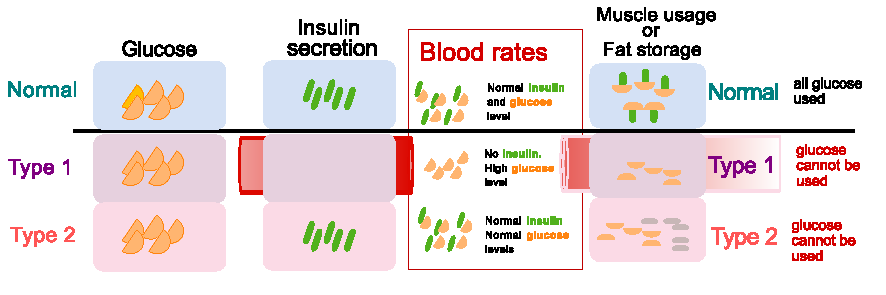
\includegraphics{diabetes_drawing}


\subsection{Energy, activities}
WRITE OR PASTE
\subsection{Energy Bar}
In order to give the user the most relevant feedback on how his blood sugar can affect his energy, we provided an Energy Bar item that displays the available energy. The bar is an 
\subsection{Symptoms}
WRITE OR PASTE
\subsection{Food system}

%\subsubsection{General overview}
The food object is an object that represents a food item in 3D, with a script inside to make the object eatable. The implementation of a food system that allows the representation of a diabetic avatar was designed following the created model described in section~\ref{sec:mymodelSection} and was made as generic as possible so that the model can be easily enhanced or changed. For instance the time-scale can be slowed or accelerated for glucose absorption and the effects of insulin. Similarly, any model can be used in place of the current model for the glucose/insulin changes as we only need to compute tables of values.

\begin{figure}[!h]
  \caption{Global and local parameters used in the scripts related to the feeding system}
  \centering
  \includegraphics[scale=0.45]{GLparam.jpg}
  \label{fig:GLparam}
\end{figure}

At each time, glucose level can be computed from the model according to global and local parameters as shown in figure~\ref{fig:GLparam}. These parameters are located in two scripts : StateScript and FoodObject. As described in section~\ref{}, StateScript is the main script for the avatar, controlling the glucose-insulin system and the avatar's behaviour related to diabetes such as triggering hypoglycemia or hyperglycemia symptoms. FoodObject is a generic script that describes each food item behaviour. 

According to our requirements, a minimal amount of specific features need to be implemented for each kind of food : the total amount of glucose in a food item, its name and the time needed to reach the glucose peak (maximum level of blood glucose since the food consumption). This generic skeleton is used for each food object in the simulation. The total amount of glucose is taken from tables such as~\ref{fig:foodGlucoseTable} and also from \cite{nutritiondataWebsite} 
%http://nutritiondata.self.com/
when the data can't be found in tables. \\

When a food object is touched by an avatar, it is attached to his hand, and he begins `eating' it, displaying on screen the correct animation. Then, the object is destroyed.

\iffalse

\begin{figure}[h]
  \caption{Carbohydrates in a set of food servings - Adapted from \cite{foodGlucoseTableWebsite}}
  \centering
  \includegraphics[scale=0.6]{foodGlucoseTable}
  \label{fig:foodGlucoseTable}
\end{figure}


\\
The Glycemic Index (GI) and the Glycemic Load (GL) are two measures %values
that can be found in similar tables. Used by nutritionists since 1980, the glycemic index characterizes how quickly blood glucose rises after the consumption of a specific kind of food. 
Created in the 1980s, the GI is based on a reference, usually pure glucose or white bread, valued at 100 which is the highest possible GI as shown in figure~\ref{manyGI}. 30 minutes after the food consumption, a higher GI induces a higher blood glucose peak. It can also be noticed that if the GI is between medium and high, an reactive (or postprandial) hypoglycemia is observed after 2 hours, which wouldn't be observed if the consumed food had a lower GI.

%cited ?
\begin{figure}[h]
  \caption{Glycemic index for different kind of food}}
  \centering
  \includegraphics[scale=0.6]{foodGlucoseTable}
  \label{fig:foodGlucoseTable}
\end{figure}

%tocite
\begin{figure}[h]
  \caption{Low and high GI \cite{last2006low}}}
  \centering
  \includegraphics[scale=0.6]{low-high-GI.gif}
  \label{fig:low-high-GI}
\end{figure}

If the temporal rise of blood glucose can be predicted by using GI, this index doesn't take into account the amount of ingested carbohydrates. For this purpose, the glycemic load (GL) was established to estimate how much the blood glucose will rise after eating a specific food. Knowing the food serving weight and the amount of glucose inside, this formula gives the link between the glycemic index and the glycemic load : $GL = IG * (mglucose/mfood)$
\\
Figure~\ref{fig:GL_and_GI-Chart} shows the possible values for the GI and the GL.

\begin{figure}[h]
  \caption{Glycemic index and glycemic load values, from \cite{mendozaWebsite}}}
  \centering
  \includegraphics[scale=0.6]{GL_and_GI-Chart.gif}
  \label{fig:GL_and_GI-Chart}
\end{figure}

%%%%%%%%%%%%%%%%%%%%%%
\fi

    \subsubsection{Issues about food destruction}
\label{foodDestruction}
Food destruction needed to be considered at the very beginning while creating the scripts' architecture and the links between all the different scripts. In fact, after being called by the FoodScript after the end of the animation, the llDie()~\cite{siteLSLWiki} function is called by the script to destroy the food object. This interrupts the execution of the FoodScript. As a consequence, a progressive release of glucose in the avatar's blood over the time, that is supposed to last about 2 hours, cannot be ensured by the FoodScript. Thus, the StateScript is in control of releasing the glucose in blood.\\

Furthermore, the destruction of the food object need to be synchronized with the end of the `eating' animation : if the objects dies too early, the avatar will appear as eating nothing, and if it dies too late, the food item will disappear unrealistically after the end of the eating movements, while being in the hand. This issue will be tackled in~\ref{sec:animBite}.


%explain animations, sequence of animations


	\subsubsection{Realism enhancement}
The main issue to solve with the food object was to give it a realistic behaviour, essentially on 3 points : how the action of eating the food is triggered, how to render an appropriate eating animation according to the food item and how to make the food object disappear realistically.
\\
	\paragraph{A realistic trigger for the `eat' action}
\label{sec:food}
% PUT IN BEGINNING The food object is an object that represents a food item in 3D, with a script inside to make the object eatable. 
% NON USED The food object doesn't do any calculation, but sends to the StateScript the reference values that correspond to the food. 

To trigger the action of eating the food, different solutions are possible : \\
PICTURES !

\begin{enumerate}
\item The food is eaten when the avatar right-clicks on the object to access the contextual menu, then selects the "Eat" action. The addition of a personalized command in the contextual menu was needed, and was also used for other problems. Details are discussed in~\ref{sec:menuAction}. However, this solutions is the most complicated from a user interface perspective, as it requires at least 2 clicks to eat the item.
\item The food is eaten when the avatar "walks" on the object, as in some video games. The main disadvantage of this solution is that the avatar can eat the object by mistake, if he moves back while the food object was behind him.
\item The food item is eaten when the avatar simply clicks on it. A minor problem with this solution is that there is no way to know in advance which object can be eaten if there's nothing to show that it's clickable. There is currently a text with the food name onto the object but the rendering is unattractive so the text will be removed in order to enhance realism and user experience.
%, it will be hard to detect with which object of the kitchen interactions are available.
\end{enumerate}

The third solution was chosen as it provides a good compromise between the simulation needs and the application's ergonomic. However, an improvement will be added by implementing the solution used to make the avatar sit automatically on a chair, described in section~\ref{sec:seat}.

The same analysis can be done for the action of taking insulin : the second solution is even worse when transposed the insulin injection as injecting by mistake is highly undesirable.

	\paragraph{Different animations : an animation library}
\label{sec:animLib}

According to the food objects nature, the eating animation played will be different. In fact, eating a sandwich is different of eating a bit of chocolate: in the first case, the two hands may be needed, and the animation takes longer as eating a sandwich takes more time, while in the second case, only one bite is needed.\\
SCHEMA\\

3 kinds of elementary animations were used : 
\begin{itemize}
\item An animation designed to eat a single item (like a sweet), also used to simulate a single bite when multiple bites are needed (like eating a cookie) and for plates (like eating pasta).
\item Secondary animations to cut the food, and poke the food with a fork.
\item An animation for drinking.
\end{itemize}
The first idea was to loop the elementary animations when the food objects need many bites, and for drinking. The second idea was to use combinations. 

Thus, the simple bite animation can be used for many purposes once combined with itself or with secondary animations :
\begin{itemize}
\item to eat a simple item, like a crisp
\item to eat sandwiches, by combining a right hand simple bite animation with a left hand simple bite animation
\item to eat a plate of food, by adding a first animation that cuts the food in a plate in the left hand. In the right hand, a second animation is played to take a piece of food in a plate, before playing the simple bite animation in the same hand.
\end{itemize}

For drinking, the animation was simply looped.\\

This approach, using a library of animation, can be generalized to the animations used in the insulin injection.

	\paragraph{Identification of the correct animation length to destroy objects at the right time}
\label{sec:animBite}
If possible, the food object should die when it's close to the mouth, during the latest bite. As all food items are not using the same animation while being eaten as described in section ~\ref{secDiffAnim} , the duration of the animation also needs to be stored, as an internal value for the Food script, for each kind of food. With this information, the llSleep() function can be called by the script to stop its execution during the animation, waiting for the appropriated moment to kill the object. 
Computing the appropriate moment was complicated by the rights permission that asks the user allows the food attachment to his hand, triggered after clicking on the food item. This time need to be added to the computation. Moreover, the issues explained in section~\ref{sec:animLib} about playing multiple animations or looping them need to be taken into account, and need to be added to the result.\\
Graph of the execution ? With one or two animation shown. %The animation lenght is automatically computed ... do it ?

\subsection{Insulin and glucose meter}
	\subsubsection{Insulin} 
	WRITE IT
	\subsubsection{Glucose Testing}

A glucose meter is needed inworld so that the user can know the blood glucose level and whether it's necessary to have an insulin injection or a meal to rise blood glucose. It is also a major aspect of diabetes experience in real life so users need to be familiar with it.

A glucose meter device was created in world with the Opensim builder tool shown in picture~\ref{fig:opensimBuilder}. The device can be carried in the avatar's inventory 
(which is the equivalent of keeping it in the pocket in real life) and accessible wherever the avatar can be, 
or kept somewhere in the house, on a desktop for instance, which means that the avatar needs to move there in order to test his blood glucose. 
Logs with the results of each test are the main way for the diabetes team in the hospital to follow the day to day evolution of diabetes, in order to improve diabetes management and to adapt the treatment to the patient's needs. \\

For this purpose, the glucose meter object displays in world the result of the test each time it's used. \\
The first solution is to send an HTTP request to the server to retrieve from the database the most recent value of blood glucose. 
This solution make use of the existing webserver that is used to display the energy bar on the menu, so it only needs to write a method on the server to send an HTTP response with the result. 
The problem of this implementation is that the webserver is necessary, so the glucose testing functionality won't be available in case of a demo start. \\

The second solution is to use the llSay() set of methods to communicate directly with the StateScript, used to compute the avatar's blood glucose at each moment. 
As described in figure~\{glucoseMeterCommunication} the glucose meter script sends a request to the StateScript, which sends the current value of the blood glucose.
This method is quicker (see come testing results? in the "Technical Evaluation" chapter) and allows the glucose meter to be used even if the web server crashes.\\

Indeed, in case of a server failure, this last point is especially crucial because the energy bar on the top of the screen won't display energy any more. 
Given that the main aim of the simulation is to teach users how to test, when to test and how to manage blood glucose, the software has to be able to deal with such a failure and to continue to give a way for the user to know the blood level so that it can still be corrected. \\

For this reason, the second solution was chosen so that there is still a way to test blood levels and to continue using the simulation even without a web server.\\


In both cases, after receiving the value of blood glucose, this value is displayed on the meter with a llSetText.  The glucose meter script is also responsible for keeping for logging the values of all the previous blood tests realized by the user. The logs are stored locally in a list (only the dozen of last values), and also sent to the web server database. 
It is possible to consult the full logs to know whether the testing is done as often as it should be. The Logs web page was realized for this purpose, using the web server and it's database with the complete results.
\subsection{General issues}

%This section describes the features implementation. choices and a travers l'implementation des features, je vais décrire des problemes plus generaux, les solutions apportées à ces problemes et les demarches employées pour les résoudre.//

%vais decrire des problemes relatifs à ... et la demarche pour//
	\paragraph{Seating}
		\label{sec:seat}
Give the examples of the sit on chair/bed and food click.
		
	\paragraph{Adding an action in the contextual menu}
	\label{sec:menuAction}
Give the example of the boat (Fish !) and the eat actions\\
We can add a personalized action to be executed when selected in the contextual menu~\ref{contextMenu}. The added action will replace the original default action, a "Sit" action that makes the avatar sit on the object. It is a default action allowed for any physical object by Opensim, even if the sitting action and the sitting point (see section~\ref{sittingpoint} for details on the sitting point) aren't already defined by the user for the object. 
\\For some reasons, we may want to make another action available from the contextual menu instead of the Sit action. The number of buttons in the contextual menu is fixed, so the only way to do so it to replace the Sit button. First step is to change the action executed when clicking on the button. This can be done by scripting, calling the llSetSitText() function. 

%%%%%%%%%%%%%%%%%%%%%%%%%%%%%%
	%uncomment
	%\subsubsection{Orientation and position issues related to the animation's constraints}
	%comment
	\paragraph{Orientation and position issues related to the animation's constraints}

\paragraph{A position issue: the exemple of the fishing activity}
\label{sittingpoint}

Set the fishing animation.
The sitting point has to be defined, which means that any time someone sits on the boat, the avatar will be sitting at the same point, with the same body orientation. If not defined, the sitting point can be anywhere on the boat as shown in figure~\ref{fig:goodSittingPoint, fig:wrongSittingPoint}, which means that the avatar position won't match the animation. It is an important issue because there won't be any realism in this case, and the user may even not recognize the played animation.

\paragraph{An orientation issue: the Eating example}
When eating a food item as described in section~\ref{sec:food}, the food item is put in the avatar's hand, and the corresponding animation is played. For this purpose, the food item need to be placed correctly in the hand, to make it realistic. However, as shown with the glass in figure~\ref{fig:badFoodOrientation, fig:goodFoodOrientation}, this position is often not compatible with the one originally used to display the food in world, here a glass placed upright on the table.
For this purpose, two solutions can be used : 
\begin{enumerate}
\item Changing the object's position by using the llSetPosition~\cite{llSetPositionWebsite} in a script to change the orientation of the object depending on whether it is attached to an avatar or on the table. 
\item Using a "display only" object that is also used for automatic objects creation. The idea here is, for a set of brownies for instance, to create an "aggregate" of brownies, such as 7 or 8 pieces of cake on a plate.
This solution is especially convenient for some kind of food items, as it provides a way to generate automatically food when it is used. Disadvantage : the solution doesn't work for any kind of objects : creating an aggregate of pasta plates is not a good solution because a user usually wants to eat one item of this kind of food. There is also a problem as the food won't disappear from the plate when taken and eaten, which might look weird for an aggregate with a small number of objects displayed.  
The aggregate is created by arranging several food objects in the desired display, and then linking them into a "super object", the aggregate. As shown in figure~\ref{fig:aggregate}, Opensim make the aggregate appear as a single object. Thus, normal properties of objects are usable, in particular the object's inventory. Other objects can be put in the inventory and used by the scripts, so the object we want to give to the avatar (for instance, a piece of brownie with the orientation that matches the eating animation with the brownie held in the avatar's hand) can be put in this inventory and given by the main script of the aggregate to the avatar. The attachToAvatar~\cite{llAttachToAvatarWebsite} function is called for this purpose, and gives a copy of the brownie in the aggregate's inventory to the avatar. 
\end{enumerate}

Maybe explain when each solution is better and when I also used them ?

%%%%%%%%%%%%%%%%%%%%%%%%%%%%%%%%%%%%%%%%%%%%%%%%%
\subsection{Materials for diabetes self-education}
A complete module of the application is dedicated to improve the user's knowledge about diabetes. Learning, and testing the knowledge are the two aspect of the educational module.

A room is dedicated to improve the knowledge about diabetes. The avatar can teleport to this room, whose walls are covered by screens objects of 3 kinds :
\begin{itemize}
\item Theoretical knowledge about diabetes, displayed on web pages
\item Practical skills about insulin therapy and blood testing, in(?) the form of videos
\item Tests, displayed on web pages
\end{itemize}

The materials comes from leaflets and tests used with young patients during the nurse and dietician sessions, all of them provided by the Royal Children's Hospital of Manchester. Videos are directly streamed from Youtube, and some other informations are provided by displaying websites such as diabetes.co.uk.\\

\pargraph{Tests}
Before taking a test, users are given the web pages that contain what they should know in order to be able to answer correctly. After taking the test, they are advised to visit the page that contains the answer of the question that was missed.\\
Tests can be taken in normal or learning mode. The normal mode only displays if the answer was correct, and invites the user to answer again the missed questions after reading the related materials, while in the learning mode, the questions are directly corrected during the test, showing the correct answer for each question. 
In the first case, the user need to be able to answer correctly in order to complete the test. The second one is more useful to learn new informations about diabetes, for those that don't want to read the materials.\\

The tests are stored in the django database. For each question, different answers are provided, and one is identified as the correct one. Each question is associated with the address of the web page explaining the concepts(?) treated(?). %it deals with
A screen object is used to display the web pages, using the script used for the Energy Bar.